\chapter{Analysis of an interesting AME region: $\lambda$~Orionis}


 \section{An intereesting AME region}
  \paragraph{Justification for selection}
		The molecular ring \footnote{Also known as the Meissa Ring}, \citep{maddalena86,maddalena87} around $\lambda$~Orionis exhibits AME with a resolvable topology even at ~1$^{\circ}$ angular resolution.
    The region is shown in Fig. \ref{fig:orionis-akari9} as it appears in 1$^{\circ}$-smoothed A9 data\footnote{Images at each wavelength used here are included as in appendix to this thesis}. The ring structure itself indicates excess microwave emission attributed to AME while the central region is dominated by free-free emission \citep{aran09, koenig15,planck15XXV}. The central region is heated by the $\lambda$ Orionis star itself, and the Orion OB association it belongs to \citep{ochsendorf15}. At approx. 10$^{\circ}$ wide, we can see the outline of the structure even in the low (1$^{\circ}$ FWHM) resolution PCAME map. The ring shape itself is thought to originate from a supernova \citep{aran09}.

  \paragraph{A well-studied region}
    The LOri region \footnote{Orion-Eridanus superbubble, Meissa ring} has been a popular target for study. Many works have investigated the astrophysics of individul portions of this region. A much smaller number of works have examined the entire ring structure as whole. The large angular size is such that all-sky surveys, especially WISE \citep{koenig15}, became a natural source of insight. The region was strongly highlighted by a Planck Collaboration microwave foregrounds follow-up investigation, as strong candidate for further AME investigation \citep{planck15XXV}.

		\paragraph{Investigative approach}
			In order to shift towards an investigation of individual AME-prominent regions, we have carried out an initial comparison of the AME of this region with its mid to far-IR dust emission.

		\paragraph{Data preparation}
			As indicated in Ch. \hyperref[ch:datasources]{\ref{ch:datasources}}, we use 12 photometric all-sky maps. For the IRC data (A9 and A18), we produce mosiacs of LOri from the individual tiles provided in the internal all-sky archive.\footnote{IRC all-sky data is still in the proprietary phase at the time of this writing, but should be public by April 2018.} For the other sources, HEALPix all-sky maps are available publicly, at sufficient resolution relative to their native resolutions. \footnote{Planck data was retreived from the NASA IPAC online archive at \url{http://irsa.ipac.caltech.edu/data/Planck/release_2/all-sky-maps/}}\footnote{AKARI/FIS data }\footnote{IRAS/IRIS data }

		\paragraph{Extraction from HEALPix maps}
		  For the data obtained via HEALPix maps, we employ the ``healpix2wcs'' functionality provided in the ``gnomdrizz'' python package\footnote{Available at \url{http://cade.irap.omp.eu/dokuwiki/doku.php?id=software}}\footnote{``drizzlib'' 1.2.2 and earlier were not able to correctly access HEALPix files with multiple fields/columns. See appendix for our recommended workaround.} A9 and A18 images are produced by regridding the images with the ``montage'' software by NASA/IPAC

		\paragraph{Multi-wavelength characterization}
			Figure \ref{fig:orionis-img} shows the region in 12 photometric bands, from the mid to far IR. Contours indicate the region's shape in the PCAME map. Figure \ref{fig:orionis-corr} shows IR to AME cross correlation plots, for all pixels within the 10$^{\circ}$ by 10$^{\circ}$ $\lambda$~Orionis region. The correlation is most clear for the shortest and for the longest wavelength bands, and weakens the most at around 60~$\mu$m. The weakening of the correlation score appears to come from brighter 25 to 90~$\mu$m emission within the ring. The spectrum is consistent with warm thermal dust emission, heated by $\lambda$~Orionis itself, and other nearby OB stars. The ring structure itself appears relatively consistent accross all bands.

		\paragraph{Ionization fraction}
			We attempt to estimate the relative fraction of charged to neutral PAHs via the R(A9:I12) band ratio. A9 is known to cover ionized PAH features (as well as neutral) whereas I12 primarily covers neutral features.
      %Fig. \ref{fig:lori_RA9I12} indicates that R(A9:I12) correlates with $AME_{var}$

\begin{figure*}
  \label{fig:orionis-akari9}
  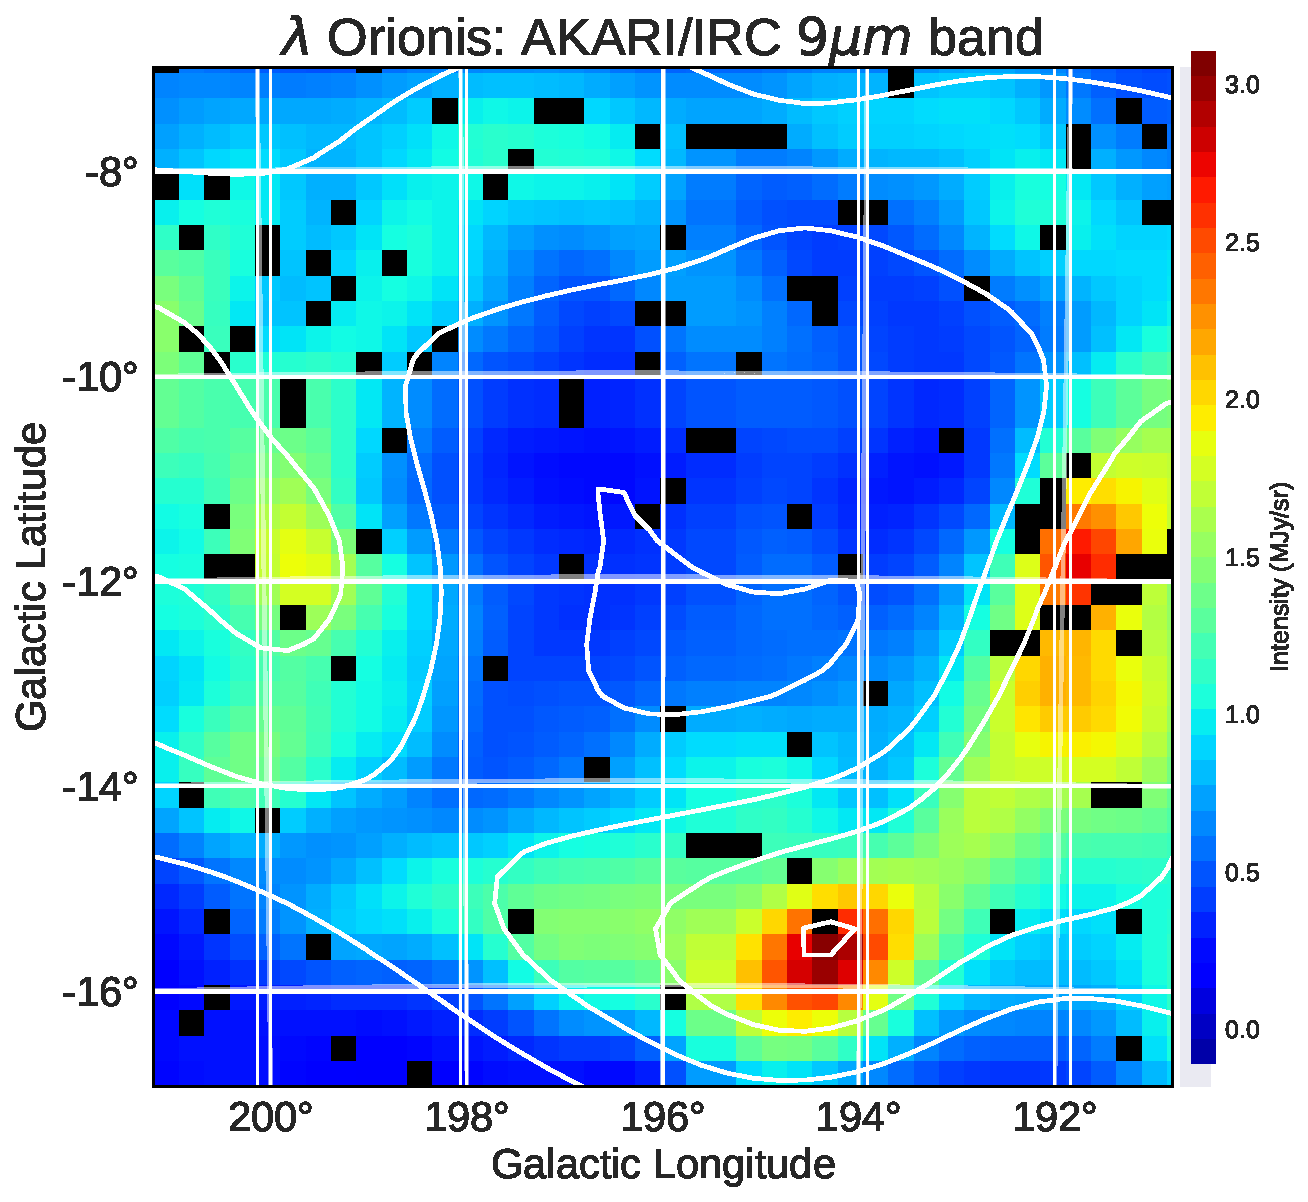
\includegraphics[width=150mm]{../Plots/LOri_akari9_AMEcont_1dres.pdf}
  \centering
  \caption{$\lambda$~Orionis as it appears in the AKARI 9~$\mu$m data. Contours indicate the AME, as given by the Planck PR2 AME map. The image is smoothed to a 1$^{\circ}$ PSF (much larger than the original 10 arcsec map. The $\lambda$~Orionis star itself is approximately located at the center of the image.
  %The dust wave structure, described by *citation needed*, is apparent, and seems to coincide with a local maxima in the PR2 AME contours. The units are MJy/sr. )
  }
\end{figure*}

\begin{figure*}
  \label{fig:orionis-img}
  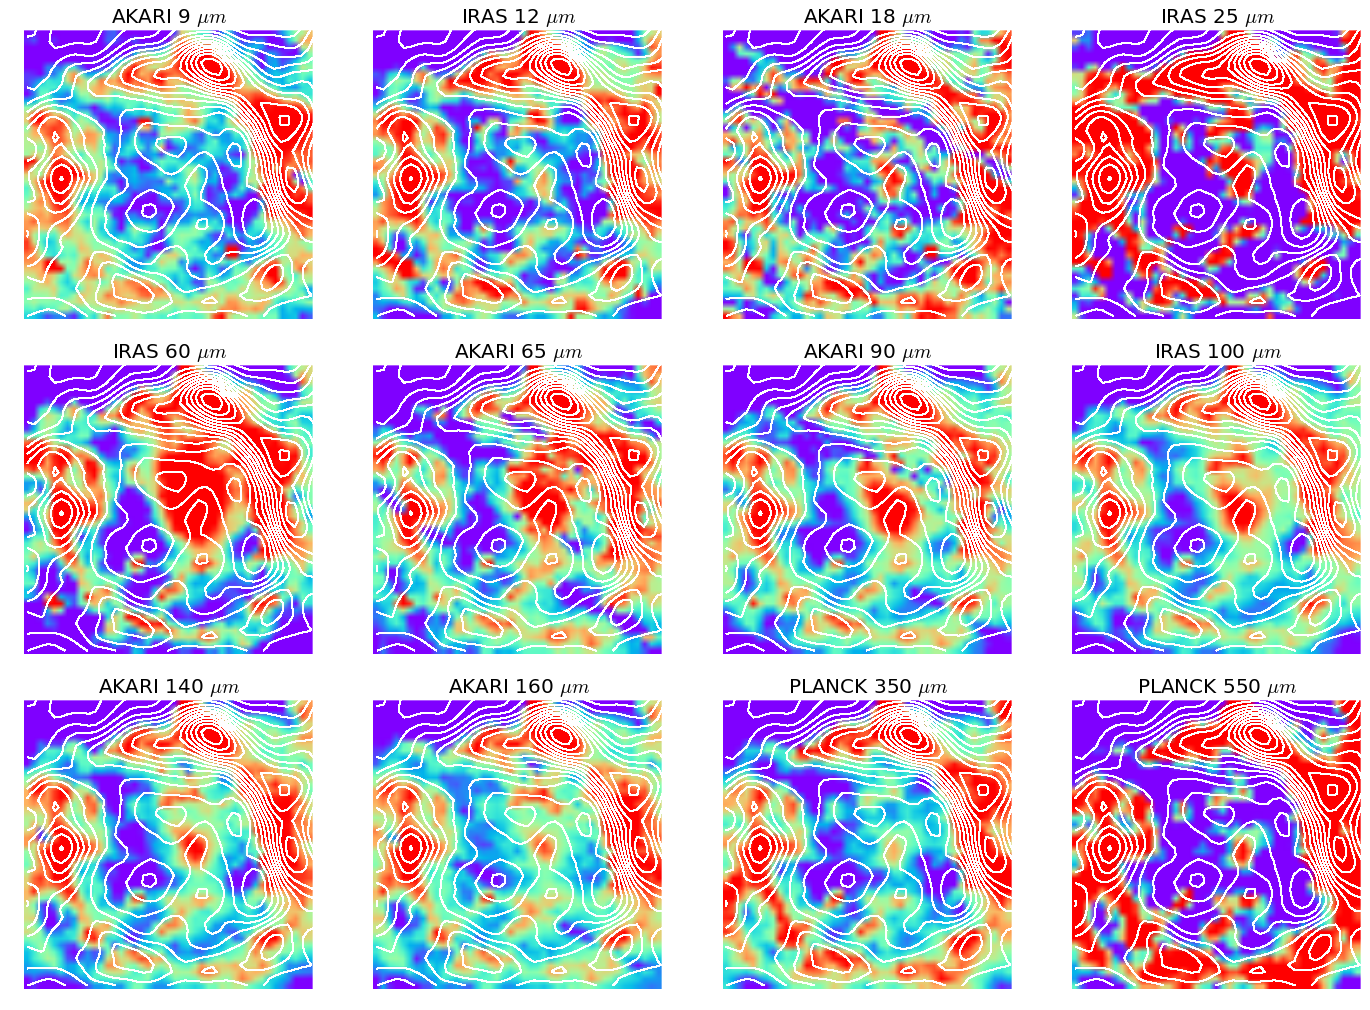
\includegraphics[width=170mm]{../Plots/lOrionis_grid_img.png}
  \centering
  \caption{A grid of thumbnails showing the $\lambda$~Orionis region's structure, at 12 wavelengths, along with AME contours (shown in white countours. Spatial correlation seems to be the best at the shortest and longest wavelengths (AKARI/IRC 9~$\mu$m and Planck/HFI 550~$\mu$m). The images are smoothed and interpolated for demonstration. Figure \ref{fig:orionis-akari9} demonstrates the actual pixel grid used for the SED fitting and intensity correlation tests.}
\end{figure*}

\begin{figure*}
  \label{fig:orionis-corr}
  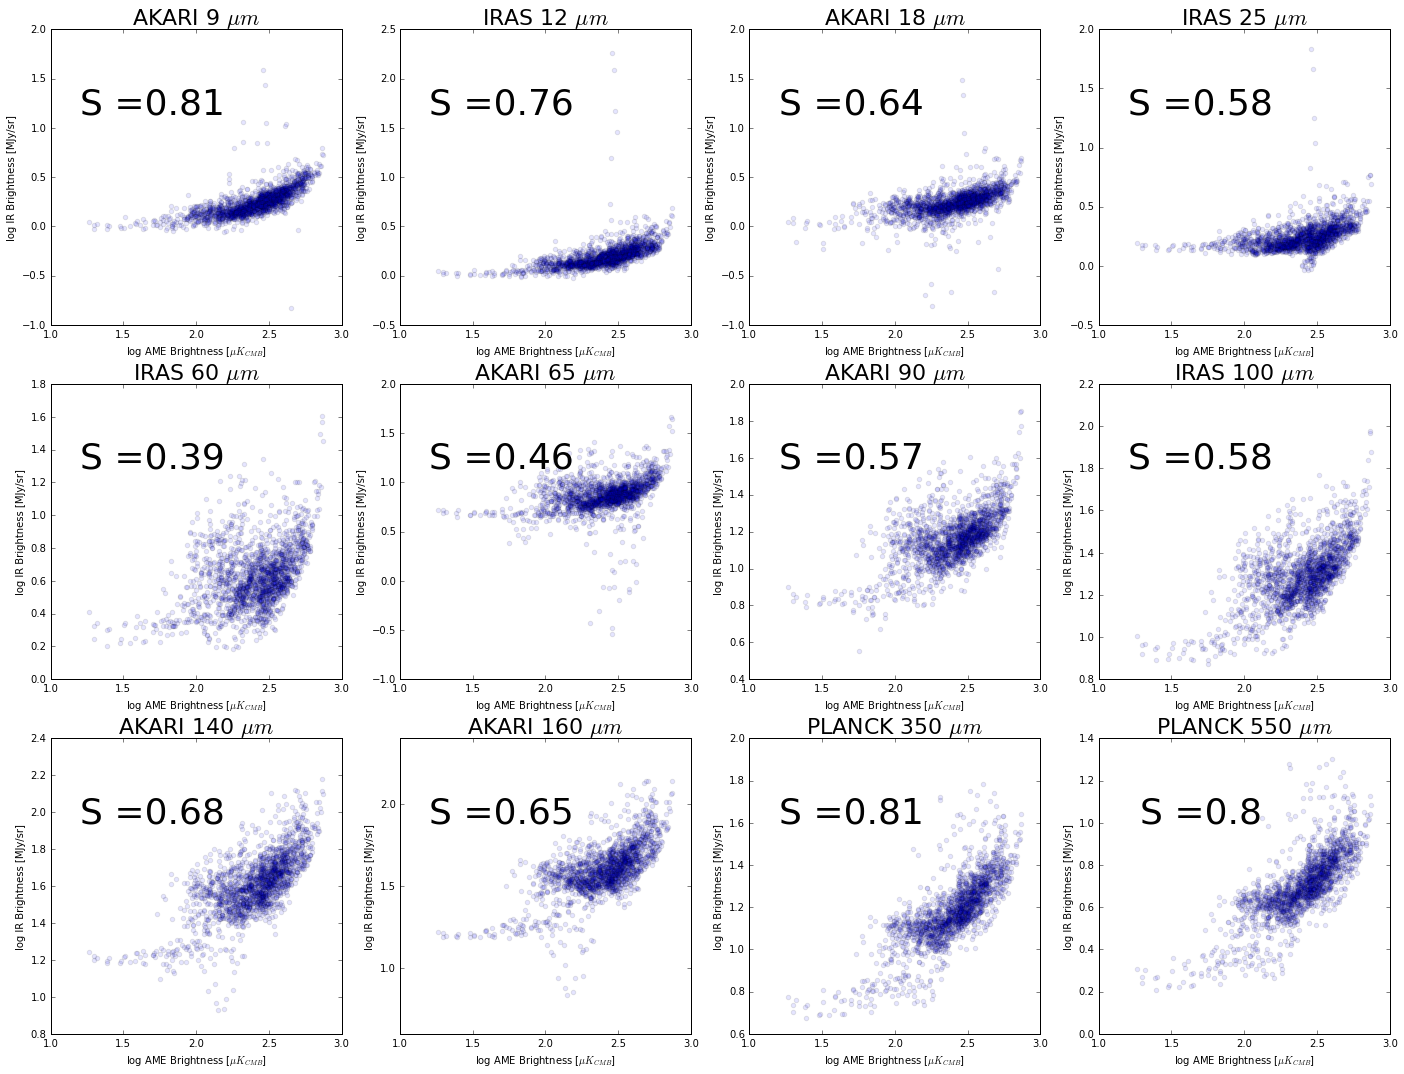
\includegraphics[width=170mm]{../Plots/orionis_correlations_AME.png}
  \centering
  \caption{Pixel cross-correlation for all pixels in the $\lambda$~Orionis cut-out region.  $S$ indicates the Spearman rank correlation coefficient for each plot.}
\end{figure*}

\subsubsection{SED Fitting}

We performed a full dust SED fitting on the LOri photometry, according to the \cite{galliano11} dust model. We used a mixture of amorphous carbon and silicate dust. Indeed, this dust mixture is more emissive than the standard silicate-graphite \citep{draine07}, by a factor of 2-3. As was shown by Herschel, in the LMC \citep{galliano11}, and by Planck, in the Milky Way \citep{planck16}, this increase of emissivity is necessary to have a proper fit of the sub-mm emission. We assume that the radiation field heating this dust mixture is the Galactic ISRF \citep{math83}, scaled by a factor $U$. We also assume, following \cite{dale01}, that the dust is exposed to a distribution of starlight intensity, distributed as:

\begin{equation}
   \label{eq:U}
     dM_{dust}\propto{} U^{-\alpha}dU
\end{equation}

between $U_{min}$ and $U_{max}$, where $U_{min}$, $U_{max}$ and $\alpha{}$ are free parameters. An old stellar population template (PEGASE; \citep{fioc97}) is added to this SED in order to model the near-IR emission. We perform a simple least-squares analysis.
